在上一节的最后一部分中,在用TableGen的语法编写完甜甜圈食谱之后,现在可以通过自定义的TableGen后端打印食谱了。

\begin{tcolorbox}[colback=blue!5!white,colframe=blue!75!black, fonttitle=\bfseries,title=Note]
\hspace*{0.7cm}请不要将\textbf{TableGen后端}与\textbf{LLVM后端}混淆:前者将TableGen文件转换(或转换)为任意文本内容,\texttt{C/C++}头文件是最常见的形式。另一方面,LLVM后端会将LLVM\textbf{中间表示(IR)}转译为底层汇编代码。
\end{tcolorbox}

本节中,我们将开发TableGen后端来打印前一节中甜甜圈食谱:

\begin{tcblisting}{commandshell={}}
=======Ingredients=======
1. oil 500 ml
2. flour 300 g
3. milk 1.25 cup
4. whole egg 1
5. yeast 1.50 tsp
6. butter 3.50 tbsp
7. sugar 2.0 tbsp
8. salt 0.50 tsp
9. vanilla extract 1.0 tsp

=======Instructions=======
1. use deep fryer to heat oil until 160 C
2. use mixer to mix flour, milk, whole egg, yeast, butter,
sugar, salt, and vanilla extract. stir in low speed.
3. use mixer to mix outcome from (step 2). stir in medium
speed.
4. use bowl to ferment outcome from (step 3).
5. use rolling pin to flatten outcome from (step 4).
6. use cutter to cut outcome from (step 5).
7. use deep fryer to fry outcome from (step 1) and outcome from
(step 6).
\end{tcblisting}

首先,\texttt{llvm-tblgen}是驱动TableGen翻译过程的程序。然后,再展示如何开发打印食谱的TableGen后端。最后,展示如何将后端集成到\texttt{llvm-tblgen}。

\subsubsubsection{4.4.1\hspace{0.2cm}TableGen的高层工作流}

TableGen后端接受我们刚刚学习的TableGen代码的内存表示(以\texttt{C++}对象形式),并将其转换为任意文本内容。整个过程由\texttt{llvm-tblgen}可执行文件驱动,其工作流程如图所示:

\hspace*{\fill} \\ %插入空行
\begin{center}
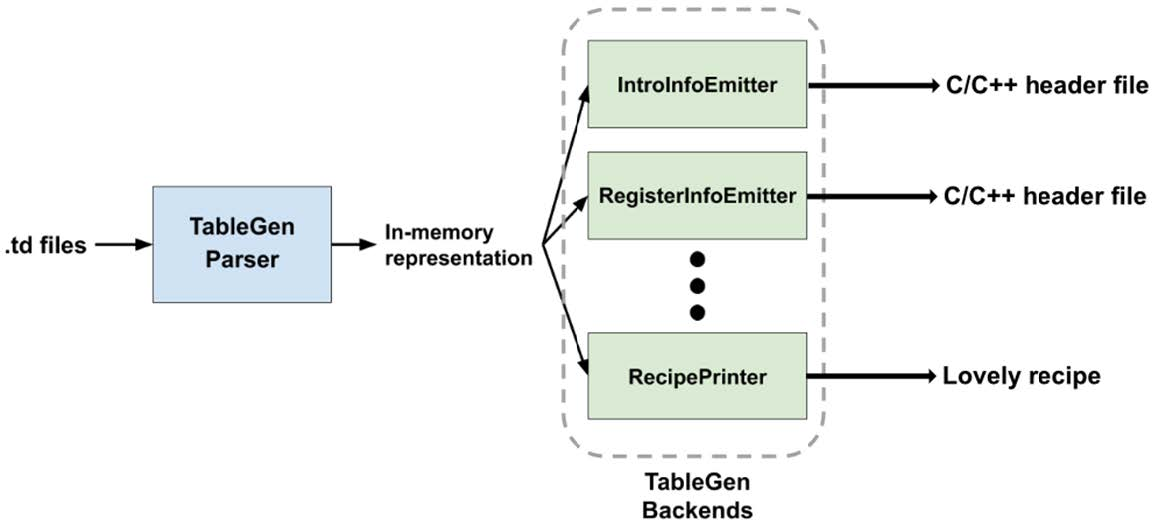
\includegraphics[width=0.9\textwidth]{content/1/chapter4/images/1.jpg}\\
图4.1 - llvm-tblgen工作流程
\end{center}

TableGen代码的内存表示(由C++类型和API组成)在TableGen后端开发中扮演着重要的角色。与LLVM IR类似,是分层组织。从顶层开始,这里有层次结构的表,每个项目都是一个C++类:

\begin{itemize}
\item \texttt{RecordKeeper}: 当前翻译单元中所有Record对象的集合(和所有者)。
\item \texttt{Record}: 表示一个记录或一个类。封闭字段由\texttt{RecordVal}表示。如果它是一个\texttt{class},也可以访问它的模板参数。
\item \texttt{RecordVal}: 表示一对记录字段及其初始值,以及字段的类型和源位置等补充信息。
\item \texttt{Init}: 表示字段的初始值。它是许多初始化值的父类,代表不同类型的初始化值——例如,\texttt{IntInit}代表整数值,\texttt{DagInit}代表DAG实例。
\end{itemize}

为了更了解TableGen后端实际完成的事情,一下是其框架结构:

\begin{lstlisting}[style=styleCXX]
class SampleEmitter {
	RecordKeeper &Records;
public:
	SampleEmitter(RecordKeeper &RK) : Records(RK) {}
	void run(raw_ostream &OS);
};
\end{lstlisting}

这个发射器接受一个\texttt{RecordKeeper}对象(由构造函数传入)作为输入,并将输出输出到\\\texttt{raw\_ostream}流中——\texttt{SampleEmitter::run}的函数参数。

下一节中,将展示如何设置开发环境,并动手编写TableGen后端。

\subsubsubsection{4.4.2\hspace{0.2cm}编写TableGen后端}

在本节中,将展示编写一个后端,用来打印使用TableGen编写菜谱的步骤。从设置开始。

\hspace*{\fill} \\ %插入空行
\noindent
\textbf{项目设置}

首先,LLVM已经提供了一个编写TableGen后端的框架。请从llvm项目的源代码树中拷贝llvm/lib/TableGen/TableGenBackendSkeleton.cpp文件到llvm/utils/TableGen文件夹中,如下所示:

\begin{tcblisting}{commandshell={}}
$ cd llvm
$ cp lib/TableGen/TableGenBackendSkeleton.cpp \
      utils/TableGen/RecipePrinter.cpp
\end{tcblisting}

然后,将\texttt{cSkeletonEmitter}类重构入\texttt{RecipePrinter}中。

\texttt{RecipePrinter}有以下工作流程:

\begin{enumerate}
\item 收集所有烘焙步骤和配料记录。
\item 使用函数以文本格式打印计量单位、温度、设备等成分。
\item 将所有烘烤步骤的DAG线性化。
\item 打印每个线性化的烘烤步骤,并使用函数来自定义打印格式。
\end{enumerate}

我们不打算涵盖所有的实现细节,因为许多后端代码实际上与TableGen(例如:文本格式和字符串处理)没有直接关系。因此,下面的小节只关注如何从TableGen的内存对象中检索信息。

\hspace*{\fill} \\ %插入空行
\noindent
\textbf{完成所有的烘焙步骤}

在TableGen后端,TableGen记录由C++类\texttt{record}表示。当我们想要检索从特定的TableGen类派生的所有记录时,可以使用\texttt{RecordKeeper}的函数\texttt{getAllDerivedDefinitions}。例如,想要获取本例中从\texttt{Step}的TableGen类派生的所有烘焙步骤记录。下面是如何使用\\\texttt{getAllDerivedDefinitions}的例子:

\begin{lstlisting}[style=styleCXX]
// In RecipePrinter::run method…
std::vector<Record*> Steps = Records.
getAllDerivedDefinitions("Step");
\end{lstlisting}

这为我们提供了一个记录指针列表,表示所有的\texttt{Step}记录。

\begin{tcolorbox}[colback=blue!5!white,colframe=blue!75!black, fonttitle=\bfseries,title=Note]
\hspace*{0.7cm}本节的其余部分中,我们将使用这种格式的\texttt{Record}(带有Courier字体)来引用\texttt{C++}对应的TableGen记录。
\end{tcolorbox}

\hspace*{\fill} \\ %插入空行
\noindent
\textbf{检索字段值}

从\texttt{Record}中检索字段值可能是最基本的操作。假设我们正在开发一个之前介绍的用于打印\texttt{Unit}记录对象的方法:

\begin{lstlisting}[style=styleCXX]
void RecipePrinter::printUnit(raw_ostream& OS, Record*
UnitRecord) {
	OS << UnitRecord->getValueAsString("Text");
}
\end{lstlisting}

\texttt{Record}类提供了一些方便的函数,例如\texttt{getValueAsString},来检索字段的值,并尝试将其转换为特定类型。这样在获取实际值之前,就不需要检索特定字段的\texttt{RecordVal}值(在本例中为\texttt{Text}字段)。类似的功能包括:

\begin{itemize}
\tt
\item Record* getValueAsDef(StringRef FieldName)
\item bool getValueAsBit(StringRef FieldName)
\item int64\_t getValueAsInt(StringRef FieldName)
\item DagInit* getValueAsDag(StringRef FieldName)
\end{itemize}

除了这些实用的函数外,有时只想检查记录中是否存在特定的字段。这种情况下,调用\\\texttt{Record::getValue(StringRef FieldName)}并检查返回值是否为空。但要注意,不是每个字段都需要初始化(可能仍然需要检查字段是否存在,但未初始化)。当这种情况发生时,可以让\\\texttt{Record::isValueUnset}帮助你。

\begin{tcolorbox}[colback=blue!5!white,colframe=blue!75!black, fonttitle=\bfseries,title=Note]
\hspace*{0.7cm}TableGen实际上使用了一个特殊的\texttt{Init}类——\texttt{UnsetInit}——来表示一个未初始化的值。
\end{tcolorbox}

\hspace*{\fill} \\ %插入空行
\noindent
\textbf{类型转换}

\texttt{Init}表示初始化值,但大多数时候我们不会直接使用,而是使用其子类。

例如,\texttt{StepOrIngredient}是一个\texttt{Init}类型对象,可以表示\texttt{Step}记录或成分记录。由于\texttt{DefInit}提供了更丰富的功能,所以可以更容易地将其转换为底层的\texttt{DefInit}对象。可以使用以下代码将\texttt{Init}类型\texttt{StepOrIngredient}转换为\texttt{DefInit}对象:

\begin{lstlisting}[style=styleCXX]
const auto* SIDef = cast<const DefInit>(StepOrIngredient);
\end{lstlisting}

还可以使用\texttt{isa<…>(…)}首先检查底层类型,或者不想在转换失败时收到异常,可以使用\texttt{dyn\_cast<…>(…)}。

\texttt{Record}表示TableGen记录,但如果能找到其父类就更好了,这将进一步获取相应字段的信息。

例如,在获取\texttt{SIDef}的基础\texttt{Record}对象后,可以使用\texttt{isSubClassOf}函数来判断\texttt{Record}是一个烘焙步骤,还是配料:

\begin{lstlisting}[style=styleCXX]
Record* SIRecord = SIDef->getDef();
if (SIRecord->isSubClassOf("Step")) {
	// This Record is a baking step!
} else if (SIRecord->isSubClassOf("IngredientBase")){
	// This Record is an ingredient!
}
\end{lstlisting}

了解底层的TableGen类,可以帮助我们以自己的方式打印记录。

\hspace*{\fill} \\ %插入空行
\noindent
\textbf{处理DAG中的值}

Now, we are going to print out the Step records. Recall that we used the dag type to represent the action and the ingredients required for a baking step. Have a look at the following code example:

\begin{lstlisting}[style=styleCXX]
def step_prep : Step<(heat:$action fry_oil:$oil, oil_
temp:$temp)> {
	let CustomFormat = "$action $oil until $temp";
}
\end{lstlisting}

Here, the highlighted dag is stored in the Action field of the Step TableGen class. So, we use getValueAsDag to retrieve that field as a DagInit object, as follows:

\begin{lstlisting}[style=styleCXX]
DagInit* DAG = StepRecord->getValueAsDag("Action");
\end{lstlisting}

DagInit is just another class derived from Init, which wasintroduced earlier. It contains some DAG-specific APIs. For example, we can iterate through all of its operands and get their associated Init object using the getArg function, as follows:

\begin{lstlisting}[style=styleCXX]
for(i = 0; i < DAG->arg_size; ++i) {
	Init* Arg = DAG->getArg(i);
}
\end{lstlisting}

Furthermore, we can use the getArgNameStr function to retrieve the token (if there is any), which is always represented in string type in the TableGen backend, associated with a specific operand, as illustrated in the following code snippet:

\begin{lstlisting}[style=styleCXX]
for(i = 0; i < DAG->arg_size; ++i) {
	StringRef ArgTok = DAG->getArgNameStr(i);
}
\end{lstlisting}

If ArgTok is empty, this means there is no token associated with that operand. To get the token associated with the operator, we can use the getNameStr API.

\begin{tcolorbox}[colback=blue!5!white,colframe=blue!75!black, fonttitle=\bfseries,title=Note]
\hspace*{0.7cm}Both DagInit::getArgNameStr and DagInit::getNameStr return the token string without the leading dollar sign.
\end{tcolorbox}

This section has shown you some of the most important aspects of working with TableGen directives' in-memory C++ representation, which is the building block of writing a TableGen backend. In the next section, we will show you the final step to put everything together and run our custom TableGen backend.

\subsubsubsection{4.4.3\hspace{0.2cm}集成RecipePrinter TableGen后端}

After finishing the utils/TableGen/RecipePrinter.cpp file, it's time to put everything together.

As mentioned before, a TableGen backend is always associated with the llvm-tblgen tool, which is also the only interface to use the backend. llvm-tblgen uses simple command-line options to choose a backend to use.

Here is an example of choosing one of the backends, IntrInfoEmitter, to generate a C/C++ header file from a TableGen file  that carries instruction set information of X86:

\begin{tcblisting}{commandshell={}}
$ llvm-tblgen -gen-instr-info /path/to/X86.td -o GenX86InstrInfo.inc
\end{tcblisting}

Let's now see how to integrate RecipePrinter source file to TableGen backend:

\begin{itemize}
\item To link the RecipePrinter source file into llvm-tblgen and add a command-line option to select it, we're going to use utils/TableGen/TableGenBackends.h first. This file only contains a list of TableGen backend entry functions, which are functions that take a raw\_ostream output stream and the RecordKeeper object as arguments. We're also putting our EmitRecipe function into the list, as follows:

\begin{lstlisting}[style=styleCXX]
…
void EmitX86FoldTables(RecordKeeper &RK, raw_ostream
&OS);
void EmitRecipe(RecordKeeper &RK, raw_ostream &OS);
void EmitRegisterBank(RecordKeeper &RK, raw_ostream &OS);
…
\end{lstlisting}

\item Next, inside llvm/utils/TableGen/TableGen.cpp, we're first adding a new ActionType enum element and the selected command-line option, as follows:

\begin{lstlisting}[style=styleCXX]
enum Action Type {
	…
	GenRecipe,
	… 
} 
…
cl::opt<ActionType> Action(
	cl::desc("Action to perform:"),
	cl::values(
		…
		clEnumValN(GenRecipe, "gen-recipe",
				   "Print delicious recipes"),
		…
	));
\end{lstlisting}

\item After that, go to the LLVMTableGenMain function and insert the function call to EmitRecipe, as follows:

\begin{lstlisting}[style=styleCXX]
bool LLVMTableGenMain(raw_ostream &OS, RecordKeeper
&Records) {
	switch (Action) {
		…
		case GenRecipe:
		EmitRecipe(Records, OS);
		break;
	}
}
\end{lstlisting}

\item Finally, don't forget to update utils/TableGen/CMakeLists.txt, as follows:

\begin{lstlisting}[style=styleCXX]
add_tablegen(llvm-tblgen LLVM
	…
	RecipePrinter.cpp
	…)
\end{lstlisting}

\item That's all there is to it! You can now run the following command:

\begin{tcblisting}{commandshell={}}
$ llvm-tblgen -gen-recipe DonutRecipe.td
\end{tcblisting}

(You can optionally redirect the output to a file using the -o option.)

The preceding command will print out a (mostly) normal donut recipe, just like this:

\begin{tcblisting}{commandshell={}}
=======Ingredients=======
1. oil 500 ml
2. flour 300 g
3. milk 1.25 cup
4. whole egg 1
5. yeast 1.50 tsp
6. butter 3.50 tbsp
7. sugar 2.0 tbsp
8. salt 0.50 tsp
9. vanilla extract 1.0 tsp

=======Instructions=======
1. use deep fryer to heat oil until 160 C
2. use mixer to mix flour, milk, whole egg, yeast,
butter, sugar, salt, and vanilla extract. stir in low
speed.
3. use mixer to mix outcome from (step 2). stir in medium
speed.
4. use bowl to ferment outcome from (step 3).
5. use rolling pin to flatten outcome from (step 4).
6. use cutter to cut outcome from (step 5).
7. use deep fryer to fry outcome from (step 1) and
outcome from (step 6).
\end{tcblisting}

\end{itemize}

In this section, we have learned how to build a custom TableGen backend to transform a recipe written in TableGen into normal plaintext format. Things we learned here include how llvm-tblgen, the driver of translating TableGen code, works; how to use the TableGen backend's C++ APIs to operate TableGen directive's in-memory representation; and how to integrate our custom backend into llvm-tblgen in order to run it. Combining the skills you learned in this chapter and in the previous one, you can create a complete and standalone toolchain that implements your custom logic, using TableGen as a solution.













































